\documentclass[a4paper,11pt]{article}
\pagenumbering{arabic}

\renewcommand*{\familydefault}{\sfdefault}
\renewcommand\footnotemark{}
\renewcommand\footnoterule{}

\setlength{\parindent}{0mm}
\setlength{\skip\footins}{0mm}
\setlength{\footnotesep}{0mm}

\usepackage[utf8]{inputenc} 
\usepackage[inner=20mm,outer=20mm,top=10mm,bottom=20mm,marginparsep=2mm,marginparwidth=8mm]{geometry} 
\usepackage[magyar]{babel}
\usepackage{longtable}
\usepackage[usenames, dvipsnames]{xcolor}
\usepackage{colortbl}
\usepackage[colorlinks=true, linkcolor=blue]{hyperref}
\usepackage{enumitem}
\usepackage{pdfpages}
\usepackage{auto-pst-pdf}

\usepackage[nomessages]{fp}
\usepackage{multido}
\usepackage{pstricks}
\usepackage{caption}
\usepackage{xstring}
\usepackage{stringstrings}
\usepackage{ifthen}
\usepackage{xspace}
\usepackage{makeidx}

\makeindex


\usepackage[nomessages]{fp}
\usepackage{multido}
\usepackage{pstricks}
\usepackage{caption}
\usepackage{xstring}
\usepackage{stringstrings}
\usepackage{ifthen}

\linethickness{0.01mm}

\newcommand\blfootnote[1]{%
  \begingroup
  \renewcommand\thefootnote{}\footnote{#1}%
  \addtocounter{footnote}{-1}%
  \endgroup
}

\newcommand{\HRule}{\rule{\linewidth}{0.5mm}}%

\newcommand{\FPmodulo}[2]{%
  \FPeval{\modulo}{trunc(#1-(#2*trunc(#1/#2,0)),0)}%
}%

\newcommand{\uind}[1]{%
  \raisebox{0.7ex}{{\scalefont{0.7}#1}}%
}%

\newcommand{\lind}[1]{%
  \raisebox{-0.4ex}{{\scalefont{0.7}#1}}%
}%

\newcommand{\notestr}[1]{%
  \IfDecimal{#1}{%
    \FPmodulo{#1}{12}%
    \FPeval{\noteposition}{trunc(\modulo,0)}%
    \substring[v]{CCDDEFFGGAAH}{\noteposition}{\noteposition}%
    \IfEq{\noteposition}{2}{\uind{$\sharp$}}{%
      \IfEq{\noteposition}{4}{\uind{$\sharp$}}{%
        \IfEq{\noteposition}{7}{\uind{$\sharp$}}{%
          \IfEq{\noteposition}{9}{\uind{$\sharp$}}{%
            \IfEq{\noteposition}{11}{\uind{$\sharp$}}{}}}}}%
  }{%
    \IfSubStr{#1}{b}{%
      \StrSubstitute{#1}{b}{}[\keya]%
      \keya\uind{$\flat$}%
    }{%
      \IfSubStr{#1}{s}{%
        \StrSubstitute{#1}{s}{}[\keya]%
        \keya\uind{$\sharp$}%
      }{#1}%
    }%
  }%
}%

\newcommand{\note}[1]{%
  \textbf{\notestr{#1}}%
}%

\newcommand{\snote}[1]{%
  {%
    \scalefont{0.6}\notestr{#1}%
  }%
}%

\newcommand{\fretnote}[2]{%
  \IfDecimal{#1}{%
    \IfDecimal{#2}{%
      \FPeval{\noteposition}{trunc(#2 + #1*5 - trunc(#1/4,0) + 5,0)}%
      \snote{\noteposition}}{}}{}%
}%

\newcommand{\key}[1]{%
  \textbf{\notestr{\ignorespaces#1\ignorespaces}}%
}%

\newcommand{\chord}[1]{%
  \StrMid{#1}{2}{2}[\secondchar]%
  \IfSubStr{bs}{\secondchar}{\StrLeft{#1}{2}[\keynote]}{\StrLeft{#1}{1}[\keynote]}%
  \StrBehind{#1}{\keynote}[\chordid]
  \key{\keynote}%
  \StrSubstitute{\chordid}{b}{$\flat$}[\uida]%
  \StrSubstitute{\uida}{s}{$\sharp$}[\uidb]%
  \StrSubstitute{\uidb}{o}{\O}[\uidc]%
  \IfSubStr{\uidc}{mmaj}{%
    \StrSubstitute{\uidc}{mmaj}{maj}[\uidd]%
    \lind{m}\hspace*{-0.5ex}$\backslash$\hspace*{-0.5ex}\uind{\uidd}%
  }{%
    \IfSubStr{\uidc}{maj}{%
      \uind{\uidc}%
    }{%
      \IfSubStr{\uidc}{m}{%
        \StrSubstitute{\uidc}{m}{}[\uidd]%
        \IfStrEq{\uidd}{}{\lind{m}}%
        {\lind{m}\hspace*{-1.3ex}\uind{\uidd}}%
      }{%
        \uind{\uidc}%
      }%
    }%
  }%
}%

\newcommand{\scale}[2]{%
  \chord{#1}{#2}%
}%

\newcommand{\chordcircle}[3]{%
  \begin{pspicture}(3.5cm,3.5cm)%
  \def\cx{0}%
  \def\cy{5}%
  \def\outercircle{1.5}%
  \def\rnotecircle{0.23}%
  \FPeval{\innercircle}{\outercircle-\rnotecircle*2}%
  \pscircle[fillstyle=solid,linewidth=0.01,linecolor=black](\cx,\cy){\outercircle}%
  \pscircle[fillstyle=solid,linewidth=0.01,linecolor=black](\cx,\cy){\innercircle}%
  \multido{\i=270+30,\r=0+1 }{24}{%
    \FPeval{\z}{trunc(\r+1,0)}%
    \substring[q]{#1}{\z}{\z}%
    \FPeval{\octave}{\outercircle-trunc(\r/12, 0)*\rnotecircle*2}%
    \IfEq{\thestring}{.}{%
    \rput{-\i}(\cx,\cy){%
      \rput(\octave,0){%
        \pscircle[fillstyle=solid,linewidth=0.01,fillcolor=black]{0.05}%
      }%
    }%
    }{% 
      \rput{-\i}(\cx,\cy){%
        \rput(\octave,0){%
          \pscircle[fillstyle=solid,linewidth=0.01,linecolor=black]{\rnotecircle}%
        }%
      }%
      \rput{-\i}(\cx,\cy){%
        \rput{\i}(\octave,0){%
          {\snote{\z}}%
        }%
      }%
    }%
  }%
  \rput(\cx,\cy){\chord{#2}{#3}}%
  \end{pspicture}%
  \hspace*{8mm}%
  \vspace*{0.3mm}%
}%

\newcommand{\chordtable}[3]{%
  \begin{pspicture}(5cm,5cm)%
  \def\w{2.7}%
  \def\h{3.3}%
  \FPeval{\dw}{\w/5}%
  \FPeval{\dh}{\h/5}%
  \FPeval{\nx}{\w/2}%
  \FPeval{\ny}{\h+\dh/2}%
  \rput(\nx,\ny){\chord{#1}}%
  \FPeval{\nx}{\dw/-0.3}%
  \FPeval{\ny}{\dh*5}%
  \rput(\nx,\ny){\small $#2$}%
  \multido{\i=0+1}{6}{%
    \FPeval{\cx}{\i*\dw}%
    \FPeval{\cy}{\i*\dh}%
    \psline[linewidth=0.01](\cx,0)(\cx,\h)%
    \psline[linewidth=0.01](0,\cy)(\w,\cy)%
  }%
  \multido{\i=0+1}{30}{%
    \FPmodulo{\i}{6}%
    \FPeval{\st}{trunc(\modulo,0)}%
    \FPeval{\fr}{trunc(\i/6,0)}%
    \FPeval{\xpos}{\st*\dw}%
    \FPeval{\ypos}{4.5*\dh-\fr*\dh}%
    \FPeval{\fr}{trunc(#2 + \fr,0)}%
    \FPeval{\spos}{trunc(\i+1,0)}
    \substring[q]{#3}{\spos}{\spos}%
    \IfEq{\thestring}{.}{}{%
      \FPeval{\yu}{\ypos-\dh/4}%
      \FPeval{\yl}{\ypos+\dh/4}%
      \FPeval{\xs}{\xpos-\dw/2}%
      \FPeval{\xe}{\xpos+\dw/2}%
      \psframe[fillstyle=solid,fillcolor=white,linecolor=white](\xs,\yu)(\xe,\yl)%
      \IfEq{\thestring}{-}{%
        \psline[linewidth=0.03](\xs,\yu)(\xe,\yu)%
        \psline[linewidth=0.03](\xs,\yl)(\xe,\yl)%
      }{%
        \IfEq{\thestring}{X}{%
          \rput(\xpos,\ypos){X}%
        }{%
          \rput(\xpos,\ypos){\small\textbf{\thestring}\fretnote{\st}{\fr}}%
          \psline[linewidth=0.03](\xs,\yu)(\xe,\yu)%
          \psline[linewidth=0.03](\xs,\yl)(\xe,\yl)%
        }%
      }%
    }%
  }%
  \end{pspicture}%
  \hspace*{8mm}%
  \vspace*{0.3mm}%
}%

\newcommand{\fretboard}[3]%
{%
  \ifthenelse{\equal{#1}{}}{}{%
    \ifthenelse{\equal{#2}{}}{%
      \vspace*{1mm}#1~\\\vspace*{1mm}%
    }{}}%
  \begin{pspicture}(\linewidth,2.5cm)%
  \def\frets{16}%
  \def\dx{1.0}%
  \def\dy{0.4}%
  \def\disp{0.3}%
  \FPeval{\midy}{\dy * 2}%
  \FPeval{\notes}{trunc(\frets * 6,0)}%
  \FPeval{\sys}{0 - \dy/2 - 0.05}%
  \FPeval{\sye}{5*\dy - \dy/2 + 0.05}%
  \FPeval{\sxs}{\dx - \disp}%
  \multido{\i=0+1}{\frets}{%
    \FPeval{\sxs}{\i*\dx + \dx - \disp}%
    \psline[linewidth=0.01](\sxs,\sys)(\sxs,\sye)% 
    \ifthenelse{\equal{\i}{5}}{%
      \FPeval{\dotx}{\sxs - \dx*0.5}%
      \pscircle[fillstyle=solid, fillcolor=gray, linecolor=gray](\dotx,\midy){0.1}%
    }{}%
    \ifthenelse{\equal{\i}{7}}{%
      \FPeval{\dotx}{\sxs - \dx*0.5}%
      \pscircle[fillstyle=solid, fillcolor=gray, linecolor=gray](\dotx,\midy){0.1}%
    }{}%
    \ifthenelse{\equal{\i}{0}}{%
      \psline[linewidth=0.06](\sxs,\sys)(\sxs,\sye)% 
    }{}%
    \ifthenelse{\equal{\i}{12}}%
    {%
      \psline[linewidth=0.06](\sxs,\sys)(\sxs,\sye)% 
    }{}%
  }%
  \multido{\i=0+1}{6}%
  {%
    \FPeval{\sys}{\i*\dy - \dy/2}%
    \FPeval{\str}{0.04 - \i*0.005}%
    \psline[linewidth=0.01](0,\sys)(\textwidth,\sys)%
  }%
  \multido{\i=0+1}{\notes}%
  {%
    \FPmodulo{(\i)}{\frets}%
    \FPeval{\disp}{trunc(\frets*(5-trunc(\i/\frets,0)) + \modulo + 1,0)}%
    \substring[q]{#3}{\disp}{\disp}%
    \FPmodulo{(\i)}{\frets}%
    \IfEq{\thestring}{.}{}%
    {%
      \FPeval{\fre}{\modulo}%
      \FPeval{\stri}{trunc(\i/\frets,0)}%
      \FPeval{\xc}{\dx*\fre + 0.05}%
      \FPeval{\yc}{\dy*(\stri - \dy/2)}%
      \rput[tl](\xc,\yc){%
        \psframebox[fillstyle=solid,linecolor=white,framesep=0]{%
          \IfEq{\thestring}{x}{%
            \fretnote{\stri}{\fre}%
          }{%
            \small\textbf{\thestring}\fretnote{\stri}{\fre}%
          }%
        }%
      }%
    }%
  }%
  \end{pspicture}~\\%
  \ifthenelse{\equal{#1}{}}{}{%
    \ifthenelse{\equal{#2}{}}{}{%
      \vspace{-0.8cm}%
      \captionof{figure}{#1}%
      \label{#2}%
      \vspace{0.3cm}%
    }%
  }%
}%

\newcommand{\ideasubsection}[1]{%
  \subsection*{\raisebox{-0.5ex}{
\includegraphics[width=5mm]{./images/idea.pdf}}~~#1}
}

%chord shortcuts
\def\Amaj{\chord{A}}
\def\Amin{\chord{Am}}

 
% packed itemization
\newenvironment{pitemize}%
{%
  \begin{longtable}[l]{lllllllllllllllllll}%
}%
{%
  \end{longtable}%
}%

% packed enumeration
\newenvironment{penumerate}%
{%
  \begin{enumerate}[leftmargin=0.5cm]%
  \setlength{\itemsep}{1pt}%
  \setlength{\parskip}{0pt}%
  \setlength{\parsep}{0pt}%
}%
{%
  \end{enumerate} %
}%

% chord type table
\newenvironment{chords}[1]%
{
  \begin{longtable}[l]{|p{40mm}|p{15mm}||p{5mm}|p{5mm}|p{5mm}|p{5mm}|p{5mm}|p{5mm}|p{5mm}|p{5mm}|p{5mm}|p{5mm}|p{5mm}|p{5mm}|} %
  \hline %
  \textbf{#1} & \textbf{Jel} & p & k2 & n2 & k3 & n3 & t4 & sz5 & t5 & k6 & n6 & k7 & n7 \\ %
  \hline %
  \endhead %
}%
{%
  \hline %
  & \textbf{Jel} & p & k2 & n2 & k3 & n3 & t4 & sz5 & t5 & k6 & n6 & k7 & n7 \\ %
  \hline %
  \end{longtable} %
}%

% section excercises
\newenvironment{practices}%
{%
  \subsection*{\raisebox{-0.5ex}{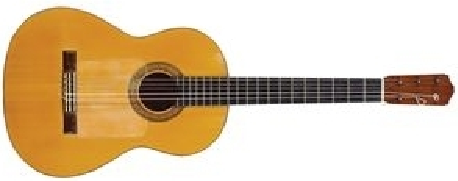
\includegraphics[width=12mm]{./images/practice.pdf}}~~Gyakorlatok}%
  \begin{penumerate} %
}%
{%
  \end{penumerate} %
}%

% Music notation
\newcommand{\aisz}{$A^\sharp$\xspace}
\newcommand{\gisz}{$G^\sharp$\xspace}
\newcommand{\cisz}{$C^\sharp$\xspace}
\newcommand{\disz}{$D^\sharp$\xspace}
\newcommand{\fisz}{$F^\sharp$\xspace}
\newcommand{\asz}{$A^b$\xspace}
\newcommand{\bebe}{$B^b$\xspace}
\newcommand{\desz}{$D^b$\xspace}
\newcommand{\esz}{$E^b$\xspace}
\newcommand{\gesz}{$G^b$\xspace}
\def\sdim{\oslash\xspace}
\def\dim{O\xspace}
\newcommand{\sst}{$\frac{1}{2}$}
 

\begin{document}

\begin{titlepage}
\begin{center}

\vspace*{1cm}
\HRule \\
\vspace*{3cm}
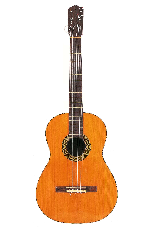
\includegraphics[width=0.20\textwidth]{./images/guitar.pdf}~\\
\vspace*{3cm}
\textsc{\LARGE Elmélet és Gyakorlat}\\[0.5cm]
\textsc{\LARGE Jegyzet}\\[0.5cm]
\textsc{\LARGE Horváth Imre gitárórái alapján}\\
\vspace*{5cm}
\begin{minipage}{0.4\textwidth}
\begin{flushleft} \large
\emph{Írta:}\\
Cserhalmi György
\end{flushleft}
\end{minipage}
\begin{minipage}{0.4\textwidth}
\begin{flushright} \large
\emph{Lektorálta:} \\
Horváth Imre
\end{flushright}
\end{minipage}
\vfill
{\large \today}
\HRule
\end{center}
\blfootnote{(c)  2013  Cserhalmi György.
Permission is granted to copy, distribute and/or modify this document under the terms of the GNU Free Documentation License, Version 1.3 or any later version published by the Free Software Foundation; with Invariant Sections being "\appendixname", no Front-Cover Texts, and no Back-Cover Texts. A copy of the license is included in the section entitled "GNU Free Documentation License".}
\end{titlepage}



\tableofcontents
\clearpage

\section*{Bevezetés}
\label{sec:bevezetes}
A következő fejezetekben zenetanulmányaimat foglalom össze a lehető legtömörebben, hozzátéve pár ötletet, 
melyekkel a saját dolgomat próbáltam megkönnyíteni. A fejezetek elméleti fejtegetéseit a mellékelt példák 
és kották teszik szemléletessé és gyakorolhatóvá. 
Ezek mellett feljegyeztem néhány, a begyakorlást segítő feladatot is. \\\\
Ez a jegyzet nem egy teljes zeneelméleti mű, inkább a megtanultak rendszerezését és ismétlését szolgáló tudástár. 
Természetesen alkalmas bizonyos fogalmak tisztázására, elvek megértésére, mégis azt javaslom, 
aki a témában el szeretne mélyülni, valamilyen formában állítson elő magának ehhez hasonló összefoglalót.


\section{Hangok, hangközök}
\label{sec:hangokhangkozok}
\subsection{Zenei hangok}
\label{sec:zeneihangok}
A zenei hang sajátossága, hogy az alaphang rezgéséhez annak felharmonikusai társulnak. Ezek összetétele határozza meg a hang színezetét. Agyunk számára olyan zenei hangok együtt-, vagy egymás után hangzása dolgozható fel kényelmesen, illetve hangzik kellemesnek, melyek felharmonikusai közel vannak egymáshoz. Bizonyíthatóan ilyenek a 6/5 (kis terc), 5/4 (nagy terc), 4/3 (tiszta kvart) illetve 3/2 (tiszta kvint) arányok. \\\\
Ebből kiindulva egy oktávnyi hangterjedelem tizenkét részre osztása terjedt el az európai zenében.
Az így felépített tiszta hangsor egymást követő elemeinek aránya nem azonos. A gitár szerkezetéből adódóan ezek az arányok enyhén eltorzultak oly módon, hogy a szomszédos osztások frekvencia viszonya $f_{h+1}/f_{h}=\sqrt[12]{2}$. Az így felépülő sort temperált (kiegyenlített) kromatikus hangsornak hívják. \\\\
A $440Hz$-es normál A hangtól indulva a kromatikus skála hangjait a következőképpen nevezzük: A, Aisz (\aisz), H, C, Cisz, D, Disz, E, F, Fisz, G, Gisz, A vagy A, Asz (\asz), G, Gesz, F, E, Esz, D, Desz, C, H, Bebé, A attól függően, hogy növekvő-, vagy csökkenő hangmagasság irányában haladunk. Oktávon túl a betűzés ismétlődik, ezeket a hangokat vesszőkkel szokás megkülönböztetni.
\subsection{Hangközök, fordított hangközök}
\label{sec:hangkozok}
Az egyszerűség kedvéért az egymást követő  hangok távolságáról szoktunk beszélni. Ebben az értelemben egy félhang távolságnak tekintjük, ha az arány közel van a $\sqrt[12]{2}$-höz. Egy hanghoz képest egy másik távolságát görög sorszámnevekkel az \ref{tab:hangkozok}. táblázatban látható módon jelöljük. Módosító jelekkel a ,,tiszta'', vagy ,,nagy'' hangközökből bővített, vagy szűkített hangközöket képezhetünk. \\\\
Általában igaz, hogy ha a hangsorban felfelé haladva $h1$ nevű hang $h2$-től  $T$ hangköznyire helyezkedik el, akkor $h2$ és az azt követő $h1$ között $12-T$ távolság van. Ezt beláthatjuk, ha a hangok neveit egy körre rajzolva képzeljük el. Arra a kérdésre tehát, hogy mely hangtól van $h2$ $T$ távolságra úgy is válaszolhatunk, hogy a $h2$-től $12-T$ közre lévő hangtól. Például a hang, aminek tiszta kvartja \fisz az a \fisz hang tiszta kvintje. A fordított hangközök az \ref{tab:hangkozok}. táblázat utolsó oszlopában láthatók.
\begin{pitemize}
 hangköz & $\frac{f}{f_{prim}}$ & név & jel & példa (C-től) & fordított hangköz (C-ig) \\ \hline
 $0$ &                   & prím                              & p     & \note{1}   &                 \\
 $\frac{1}{2}$ & $2^\frac{1}{12}$  & kisszekund                        & k2    & \note{2}   & nagyszeptim     \\ 
 $1$ & $2^\frac{2}{12}$  & nagyszekund                       & n2    & \note{3}   & kisszeptim      \\
 $1\frac{1}{2}$ & $2^\frac{3}{12}$  & kisterc                           & k3    & \note{4}   & nagyszext       \\
 $2$ & $2^\frac{4}{12}$  & nagyterc                          & n3    & \note{5}   & kisszext        \\
 $2\frac{1}{2}$ & $2^\frac{5}{12}$  & tiszta kvart                      & t4    & \note{6}   & tiszta kvint    \\
 $3$ & $2^\frac{6}{12}$  & szűkített kvint - bővített kvart  & s5/b4 & \note{7}   & szűkített kvint \\
 $3\frac{1}{2}$ & $2^\frac{7}{12}$  & tiszta kvint                      & t5    & \note{8}   & tiszta kvart    \\
 $4$ & $2^\frac{8}{12}$  & kisszext                          & k6    & \note{9}   & nagyterc        \\
 $4\frac{1}{2}$ & $2^\frac{9}{12}$  & nagyszext                         & n6    & \note{10}  & kisterc         \\
 $5$ & $2^\frac{10}{12}$ & kiszszeptim                       & k7    & \note{11}  & nagyszekund     \\
 $5\frac{1}{2}$ & $2^\frac{11}{12}$ & nagyszeptim                       & n7    & \note{12}  & kisszekund      \\
 $6$ & $2^\frac{12}{12}$ & oktáv                             & to    & \note{13}' \\
 $6\frac{1}{2}$ & $2^\frac{13}{12}$ & kis nóna                          & k9    & \note{14}' \\
 $7$ & $2^\frac{14}{12}$ & nagy nóna                         & n9    & \note{15}' \\
 $7\frac{1}{2}$ & $2^\frac{15}{12}$ & kis decima                        & k10   & \note{16}' \\
 $8$ & $2^\frac{16}{12}$ & nagy decima                       & n10   & \note{17}' \\
 $8\frac{1}{2}$ & $2^\frac{17}{12}$ & tiszta undecima                   & t11   & \note{18}' \\
 $9$ & $2^\frac{18}{12}$ & bővített undecima                 & b11   & \note{19}' \\
 $9\frac{1}{2}$ & $2^\frac{18}{12}$ & duodecima                         & 12    & \note{20}' \\
 $10$ & $2^\frac{18}{12}$ & kis tredecima                     & k13   & \note{21}' \\
 $10\frac{1}{2}$ & $2^\frac{18}{12}$ & nagy tredecima                    & n13   & \note{22}' \\
\end{pitemize}
\captionof{table}{Hangközök elnevezése, jelölése és fordítása} 
\label{tab:hangkozok}
\subsection{A gitár fogólapja}
\label{sec:gitarfogolap}
A hathúros gitár húrjai, a leggyakoribb hangolással, felülről lefelé \textit{E, A, D, G, H} és \textit{E} hangokon szólnak. A negyedik és ötödik húr között nagy terc, míg a többi, egymást követő húr között tiszta kvart hangköz van. Mivel minden lefogás fél hang lépést jelent, így a tizenkettedik pozícióban ismét \textit{E, A, D, G, H, E} hangokat találunk. Az Antonio de Torres Jurado által a XIX. században rendszeresített klasszikus- és flamenco gitár fogólapja az \ref{fig:fogolap}. ábrán látható.\\\\
\fretboard{A klasszikus gitár fogólapja}{fig:fogolap}
          {xx.x.x.xx.x.xx.x%
           xx.x.xx.x.x.xx.x%
           x.x.xx.x.xx.x.x.%
           x.xx.x.x.xx.x.xx%
           x.xx.x.xx.x.x.xx%
           xx.x.x.xx.x.xx.x}
Az egyes lefogásokhoz tartozó hangok neve (nem a magassága) könnyen meghatározható néhány szabály alkalmazásával:
\begin{pitemize}
$-$ az ötödik, tizedik és tizenkettedik lefogásnál egész hangokat találunk  \\
$-$ az ötödik lefogás a következő húr kezdőhangja, kivéve G húrt, ahol ez fél hanggal magasabb  \\
$-$ a hetedik lefogás az előző húr kezdőhangja, kivéve a H húrt, ahol ez fél hanggal alacsonyabb \\
$-$ egy húron a tizenkettedik lefogás egy oktávnyira van, ezért a hangok neve itt a húr kezdőhangja \\
$-$ a tizedik lefogáson a húr kiszeptimje van azaz egy egész hangot kell kivonni \\
$-$ a tizenkettedik lefogás felett tizenkettő kivonásával a fenti szabályok alkalmazhatók \\
\end{pitemize}
\ideasubsection{A hangközök gyors meghatározása}
A gitár hangolása - E,A,D,G,H,E -, gyorsan megjegyezhető. Ebből a kvart - kvint távolságok két alaphang kivételével azonnal kiadódnak. Pl. A az E hang kvartja, ezért E az A hang kvintje. G kvartja nem a H, hanem a C, viszont a H kvartja az E. Nincs F és C húr, de ezek fél hangra vannak az E illetve a H hangoktól, tehát kvartjaik az \aisz illetve az F. \\\\
A szekundok és tercek megtalálása nyilván nem probléma, ugyanígy - visszafelé számolva -, a szeptimek és szextek is egyszerűen kiadódnak. Később, az akkordok felépítésénél illetve a skála fokainak zenei funkció szerinti beosztásánál ennek jó hasznát vesszük.
\begin{practices}
\item Nevezz meg egy húrt és egy lefogást, majd az ott található hang nevét!
\item Tetszőleges hanghoz találd meg a kvart- és kvint hangközöket!
\end{practices}


%\section{Skálák}
%\label{sec:skalak}
%A zenei hangokat növekvő hangmagasság szerint rendezve skálát kapunk. Tizenkét hangot véve a lehetséges kettő, vagy több hangból álló skálák száma $2^{12} - 13 = 262131$. A hangközök sorozata adja az úgynevezett skálatörvényeket, míg a hangok sorozata a skála fokait. A hangsorokat a következőképpen szokás csoportosítani:
\begin{pitemize}
diatonikus & a hangok között nincs szekundnál nagyobb távolság \\
\hline
bichord & két fokú \\
trichord & három fokú \\
tetrachord & négy fokú \\
pentachord & öt tfokú \\
hexachord & hat fokú \\
heptachord & hét fokú (pl. a dúr skála) \\\\
nem diatonikus & a hangok között szekundnál nagyobb távolság van \\
\hline
biton & két fokú \\
triton & három fokú \\
tetraton & négy fokú \\
pentaton & öt fokú (pl. a blues skála) \\
hexaton & hat fokú \\
heptaton & hét fokú  (pl. a harmonikus moll skála)\\\\
modális & a dúr skála fokain alapuló heptachord \\
\hline
ión & dúr I fok \\
dór & dúr II fok \\
fríg & dúr III fok \\
líd & dúr IV fok \\
mixolíd & dúr V fok \\
aeol & dúr VI fok (természetes moll) \\
lokriszi & dúr VII fok \\\\
tonális & a dúr skála klasszikus módosításain alapuló \\
\hline
hangnem meghatározó skálák & dúr, (harmonikus) moll és melodikus moll \\
egyéb, nevezetes skálák & spanyol moll, magyar moll, ... \\
alterált skálák & az alteráció szabályai szerint alkotott szinező skálák \\
\end{pitemize}
\subsection{Hangnem meghatározó skálák}
Bármely hangnem meghatározó skála jellemzői a következők
\begin{pitemize}
$-$ minden fokról indítható skála (skálafűzés) \\
$-$ minden fokra hangzati akkordok építhetőek \\
$-$ a skála hangjai a skála bármely akkordjára játszhatóak \\
\end{pitemize}
Az kromatikus skálából hét elemet kiválasztva az európai zenében három különböző
hangulatú sort építettek fel, melyek skálatörvényei:
\begin{pitemize}
& I & & II & & III & & & IV & & V & & VI & & & VII & \\ \hline
dúr törvény & \tiny C & 1 & \tiny D & 1 & & \tiny E &\sst & \tiny F & 1 & \tiny G & 1 & & \tiny A & 1 & \tiny H &\sst & \tiny C \\
(harmonikus) moll törvény & \tiny C & 1 & \tiny D &\sst & \tiny \disz & & 1 & \tiny F & 1 & \tiny G &\sst & \tiny \gisz & & 1\sst & \tiny H &\sst & \tiny C \\
melodikus moll törvény & \tiny C & 1 & \tiny D &\sst & \tiny \disz & & 1 & \tiny F & 1 & \tiny G & 1 & & \tiny A & 1 & \tiny H &\sst & \tiny C \\
\end{pitemize}
\captionof{figure}{Hangnem meghatározó skálák skálatörvényei} 
\label{fig:hangnemek}
Látható, hogy az azonos kulcshanggal kezdődő skálák csak a harmadik és hetedik fokukban különböznek.

\begin{practices}
\item Sorolj fel a kromatikus skála bármely hangján kezdődő dúr-, moll- és melodikus moll hangsorokat!
\item A skálákat (\ref{app:skalak}) érdemes naponta gyakorolni, mert fejlesztik az összhangot a kezek között, a pengetés pontosságát és segítenek begyakorolni az egyes hangnemekhez tartozó hangok helyét a fogólapon. Az oda-vissza játék mellett különböző minták, mint például három előre, kettő vissza is gyakorolhatók.
\end{practices}

\subsection{Alterált skálák}
Mivel az alterált skálák megértéséhez szükség van az akkordok ismeretére, a téma bővebb kifejtése az \ref{sec:Alteracio} fejezetben található, a \ref{sec:Akkordok} fejezet után.

\begin{practices}
\item Határozd meg tetszőleges dúr-, vagy moll skálák fő akkordjait!
\item Határozd meg egy hármas-, vagy négyeshangzat előfordulási helyeit a hangnem meghatározó
skálákban és az ott betöltött szerepüket (pl. G dúr a C dúr domináns akkordja).
\item Szerkessz dallamokat akkord kíséretre a funkció vertikális és horizontális szemlélete szerint!
\end{practices}

\subsection{Egyéb, nevezetes skálák}


%
%\section{Akkordok}
%\label{sec:akkordok}
%Az akkord egyidőben megszólaló legaláb három különböző hang.
Nem számít különböző hangnak a hangok bármelyikétől egy, vagy több oktáv távolságra lévő hang.
Két hang nem akkord, csak hangköz. Egy adott skálához tartozónak tekintjük a skála hangaiból felépített hangzatokat. Ezen akkordok típusát (ld. lent) a skála hangközei adják.

\subsection{Hármashangzatok}
A hármashangzatok olyan akkordok, melyek az alaphangra épülő terc és kvint hangközből állnak.
\begin{pitemize}
Név & Jelölés & Példa \\ \hline
C dúr       & $C$      & C E G \\
C bővített  & $C^+$    & C E \gisz \\
C moll      & $C_m$    & C \disz G \\
C szűkített & $C^\dim$ & C \disz \fisz \\
\end{pitemize}                                                                                                                                  

\ideasubsection{Az akkordok hangjainak gyors meghatározása}
Egyszerű hármashangzat hangjai könnyen felsorolhatók, ha a két tercet fejben felsoroljuk: 
C, D, E - E, F, G. Ez alapján a C-dúr akkord a C, E és G hangokból áll. 
Ha a alaphang félhang, akkor is érdemes a közeli egész hanggal számolni, majd mindhárom
hangot eltolni fél hanggal a megfelelő irányba.

\begin{practices}
\item Definiáld a hármashangzat fogalmát, sorold fel fajtáit, a fajták felépítését és jelölését!
\item Sorold fel tetszőleges alaphanggal egy moll-, szűkített-, bővített- és dúr hármashangzat hangjait!
\item Sorolj fel a kromatikus skála bármely hangján kezdődő dúr-, moll- és melodikus moll hangsorok fokaira épülő hármashangzatokat!
\item Határozz meg hármashangzatokat a hangjai alapján!
\end{practices}

\subsection{Négyeshangzatok}
A négyeshangzatok olyan akkordok, melyeben a hármashangzatra szeptim hangköz épül.
Mivel a szeptim az akkord skálájának hangajai között a hetedik, a négyeshangzatokat hetes akkordoknak nevezzük.
\begin{pitemize}
Név & Jelölés & Példa \\ \hline
C domináns hetes            & $C^7$           &   C E G \aisz \\
C major hetes               & $C^{maj7}$      &   C E G H \\
C moll hetes                & $C_m^7$         &   C \disz G \aisz \\
C moll major hetes          & $C_m/^{maj7}$   &   C \disz G H \\
C bővített major hetes      & $C^{maj7(5\#)}$ &   C E \gisz H \\
C félszűkített hetes        & $C^\sdim$       &   C \disz \fisz \aisz \\
C szűkített hetes           & $C^\dim$        &   C \disz \fisz A \\
\end{pitemize}                                                                                                                                  
\begin{practices}
\item Definiáld a négyeshangzat fogalmát, sorold fel fajtáit, a fajták felépítését és jelölését !
\item Sorold fel tetszőleges alaphanggal az ismert négyeshangzat fajták hangjait!
\item Sorolj fel a kromatikus skála bármely hangján kezdődő dúr-, moll- és melodikus moll hangsorok fokaira épülő négyeshangzatokat!
\item Határozz meg négyeshangzatokat a hangjai alapján!
\end{practices}

\subsection{Ötöshangzatok}
Az ötöshangzatok olyan akkordok, melyeben a négyeshangzatra oktávon túli szekund, azaz nóna hangköz épül.
Mivel a nóna az akkord skálájának hangjai között a kilencedik, az ötöshangzatokat kilences akkordoknak nevezzük.
Bővített kilences hangzat nem létezik moll, szűkített illetve félszűkített hetes alapon, mert megsértené a hangzat
hangjainak különbözőségére vonatkozó szabályt. Az alapként szolgáló négyeshangzat jelöléséből kimaradhat a hetes szám,
hiszen szeptim nélkül nem beszélhetnénk ötös hangzatról.
\begin{pitemize}
Név & Jelölés & Példa \\ \hline
C kilences                     & $C^{9}$          & C E G \aisz D \\
C bővített kilences            & $C^{9\#}$        & C E G \aisz \disz \\
C szűkített kilences           & $C^{9b}$         & C E G \aisz \cisz \\
C major kilences               & $C^{maj9}$       & C E G H D \\
C moll major kilences          & $C_m/^{maj9}$    & C \disz G \aisz D \\
C bővített major szűk kilences & $C^{maj9b(5\#)}$ & C F G H \cisz \\
...
\end{pitemize}

\subsection{Hatoshangzatok}
Az hatoshangzatok olyan akkordok, melyeben az ötöshangzatra oktávon túli kvart, azaz undecima hangköz épül.
Mivel a undecima az akkord skálájának hangjai között a tizenegyedik, az hatoshangzatokat tizenegyes akkordoknak nevezzük.
A dúr hármashangzatra épülő hatoshangzat jelölése rendhagyó - a tiszta kvart bővítés jelölése $11b$, a bővített kvarté $11$.
Bővített undecimát tartalmazó hatoshangzat nem létezik , szűkített szeptim alapon, mert megsértené a hangzat hangjainak 
különbözőségére vonatkozó szabályt. Néhány példa:
\begin{pitemize}
Név & Jelölés & Példa \\ \hline
C szűkített tizenegyes      & $C^{11b}$        & C E G \aisz D E \\
C tizenegyes                & $C^{11}$         & C E G \aisz D F \\
C moll szűkített tizenegyes & $C_m^{11b}$      & C \disz G \aisz D E \\
C moll major tizenegyes     & $C_m/^{maj11}$   & C \disz G H D F \\         
C bővített major tizenegyes & $C^{maj11(5\#)}$ & C E \gisz H D F \\
...         
\end{pitemize}

\subsection{Heteshangzatok}
Az heteshangzatok olyan akkordok, melyeben az hatoshangzatra oktávon túli szext, azaz tredecima hangköz épül.
Mivel a tredecima az akkord skálájának hangjai között a tizenharmadik, az heteshangzatokat tizenhármas akkordoknak nevezzük.
Szűkített tredecimát tartalmazó hatoshangzat csak szűkített szeptim alapon létezik.
Bővített tredecimát tartalmazó hatoshangzat csak nem bővített kvint és nagyszeptim alapon létezik.
Tiszta tredecimát tartalmazó hatoshangzat csak nagyszeptim alapon létezik. \\\\
A jelölés nem tér el az eddigiektől, az alap hatos hangzat nevéhez 13, 13b, vagz 13\# index adódik.

\subsection{Suspend akkordok}
Az alaphangra épülő tiszta kvartot és kvintet tartalmazó akkordok. 
A suspend akkord után minden esetben a hangnem tercet tartalmazó akkordja következik.
Jelölése: $C^4$

\subsection{Additional akkordok}
Olyan akkordok, melyekben a hangzatra egy nem szomszédos hangzat hangköze épül.
Hármashangzatra így nóna, undecima és tredecima épülhet az ötös-, hatos- és heteshangzatokból.
Jelölése: $C^{add7}$

\subsection{6-os akkordok}
A hatos akkordok olyan négyeshangzatok, melyekben a hármashangzatra nagy szext hangköz épül.
Jelölése és fajtái:
\begin{itemize}
\item C dúr hatos - $C^6$ (pl.: C, E, G, A)
\item C moll hatos - $C_m^6$ (pl.: C, disz, G, A)
\end{itemize}

\subsection{6/9-es akkordok}
A 6/9-es akkordok olyan négyeshangzatok, melyekben a hatos akkordra nagy nóna hangköz épül.
Jelölése és fajtái:
\begin{itemize}
\item C dúr 6/9 - $C^{6/9}$ (pl.: C, E, G, A, D)
\item C moll 6/9 - $C_m^{6/9}$ (pl.: C, disz, G, A, D)
\end{itemize}

\subsection{9/6-os akkordok}
A 9/6-es akkordok olyan hagyományos ötös hangzat-beli kilences akkordok, melyekhez díszítésképpen
egy nagy szext hangköz járul.
Jelölése és fajtái:
\begin{itemize}
\item C 9/6 - $C^{9/6}$ (pl.: C, E, G, aisz, D, A)
\item C moll 9/6 - $C_m^{9/6}$ (pl.: C, disz, G, aisz, D, A)
\item C dúr 9/6 - $C^{maj9/6}$ (pl.: C, E, G, H, D, A)
\end{itemize}



\section{A skálák fokaira épülő hangzatok}
\label{sec:skalahangzat}
A skála fokaira épülő akkordok meghatározásához meg kell vizsgálni, hogy az adott skála fokról kezdve milyen terc, kvint, szeptim, nóna, undecima és tredecima építhető egymásra. A ,,\nameref{sec:skalaakkordok}'' melléklet táblázatai alapján a hármas- és négyes hangzatok típusai, megjegyezhető formában:
\begin{pitemize}
Hangnem & Hangzat & I & II & III & IV & V & VI & VII \\ \hline
Dúr & Hármas & dúr & moll & moll & dúr & dúr & moll & szűk \\
Dúr & Négyes & maj7 & moll7 & moll7 & maj7 & dom7 & moll7 & félszűk7 \\
Moll & Hármas & moll & szűk & bőv & moll & dúr & dúr & szűk \\
Moll & Négyes & mollmaj7 & moll7 & félszűk7 & moll7 & dom7 & maj7 & szűk7 \\
Harmonikus moll & Négyes & moll & moll & bőv & dúr & dúr & szűk & szűk \\
Harmonikus moll & Hármas & mollmaj7 & moll7 & moll7 & dom7 & dom7 & félszűk7 & félszűk7
\end{pitemize}%
\captionof{figure}{A skálák fokairól induló akkord típusok} 
\label{fig:skalafokakkord}
\ideasubsection{Modális skálák akkordjai}
Amint az a \ref{fig:frigskalahangzatok}. táblázatban látszik, az egyes akkordtípusok megegyeznek a dúr skála megfelelő modális fokának akkordtípusaival. Így akárcsak a skálatörvényeket, az akkord típusokat is könnyen származtathatjuk a dúr skálából.
\begin{practices}
\item Sorold fel a hangnem meghatározó skálák fokairól induló hármas- és négyeshanzatok típusait!
\item Egy kiválaszott dúr, moll, vagy melodikus moll skálához sorold fel a fokairól induló hármas- és négyeshangzatokat!
\end{practices}


%\section{Zenei funkció}
%\label{sec:funkcio}
%Minden, egy adott hangnemen belül megszólaló hang, vagy akkord a hallgatóra hatást gyakorol. Ennek ismeretében szerkeszthető meg a zeneművek felépítése és lezárása.
\subsection{Fő akkordok, mellékakkordok}
\label{sec:foakkord}
A skála fokainak funkcióelméleti megnevezése sorra \index{tonika}tonika (I), szupertonika, mediáns, \index{szubdomináns}szubdomináns (IV), \index{domináns}domináns (V), szubmediáns és vezető hang.
A hangok és akkordok a hallgatóra három jellemző hatást gyakorolhatnak. Az első fokokon található tonika megnyugvó, a negyedik fokon a szubdomináns feszültségkeltő, a domináns pedig kirobbanó hatású.
Ezek a skála \textbf{fő akkordjai}, vagy hangjai.
A keltett érzet szempontjából ezek a ,,tercrokonság elve'' alapján helyettesíthetők olyan \textbf{mellék akkordokkal}, melyekkel két hangjuk közös. 
Ezek alapján a dúr-, moll-, és melodikus moll hangnemekben a fokok szerepe a következő táblázatban foglalható össze:
\begin{pitemize}
Funkció & A skála foka \\
\hline
Tonika & I tonika & III mediáns & VI szubmediáns \\
Domináns & III mediáns & V domináns & VII vezető \\
Szubdomináns & II szupertonika & IV szubdomináns & VI szubmediáns \\
\end{pitemize}
Négyeshangzat felett is érvényesül a két közös hang hatása, de ezt nem tercrokonságnak, hanem enharmóniának nevezzük: ha két akkordban kettő, vagy több hang közös, ezek hasonló hangzásúak - enharmonikusak. Ezen akkordok skálái és bontásai oda-vissza egymásra játszhatóak. \\\\
Dúr-, moll-, illetve melodikus moll skáláknál a szubdomináns és domináns akkordok, vagy fokok 
rendre tiszta kvart és tiszta kvint távolságra vannak a tonikától. Mivel azonban a különböző skálák fő akkordjai nem egy típusúak, a három fő akkord felismerésével a zenemű hangneme meghatározható. A fokok zenei funkciói egyéb skáláknál is értelmezve vannak, de a az előbbi megállapítás ezeknél általában nem igaz. \\\\
\begin{practices}
\item Határozd meg tetszőleges dúr-, vagy moll skálák fő akkordjait!
\item Határozd meg egy hármas-, vagy négyeshangzat előfordulási helyeit a hangnem meghatározó
skálákban és az ott betöltött szerepüket (pl. G dúr a C dúr domináns akkordja).
\end{practices}
\subsection{Zárlatok}
\label{sec:zarlatok}
Autentikus zárlat: I-IV-V-I. \\
Plagális (egyházi) zárlat: I-V-IV-I. \\
Félzárlat: \\
Álzárlat: V-IV \\
Andalúz zárlat: \\
dúrban : vi - V - IV - III, mollban i – bVII – bVI – V \\
http://en.wikipedia.org/wiki/Andalusian\_cadence

%
%\section{Skála alteráció, dallamszínezés}
%\label{sec:alteracio}
%\subsection{Horizontális értelmezés}
\label{sec:horizontalisertelmezes}
A hangok illetve akkordok hangemhez kötött, horizontális értelmezéséve szerkesztett dallammenet csakis a skála hangjait tartalmazza. Ennek módosított - alterált -, skálával való színezésére az alább ismertetett módszerek használatosak.
\subsection{Vertikális értelmezés}
\label{sec:vertikalisertelmezes}
A hangok illetve akkordok hangemtől független értelmezése. A zenemű színezése történhet oly módon, hogy az éppen kísérő akkordhoz nem a hangemnek megfelelő dallamot szerkesztünk. Ehhez egy, vagy több olyan skála hangjait kell felhasználni, amelyben az adott kísérő akkord szerepel. Lásd a ,,\nameref{sec:exdallamvert}'' példát.
\subsection{Enharmonikus kiegészítés}
\label{sec:enhkiegeszites}
\begin{pitemize}
A kísérő akkord hangjaiból álló kisebb fokszámú hangzat választása \\
A kísérő akkord kiegészítése \\
A kísérő akkorddal enharmonikus akkordban hangok cseréje \\
\end{pitemize}
\subsection{Hangcsoportok}
%\label{sec:hangcsoportok}
A dallam hangjait három csoportba soroljuk.
\begin{pitemize}
Pillér hangok -- a kísérő akkord hangjai \\
Diatonikus váltóhangok -- az alterált skála hangjai, kivéve a pillér hangok \\
Kromatikus váltóhangok -- a kísérő akkord hangjaitól legfeljebb szekund távolságra lévő hangok, amelyek nem szerepelnek a hangnemben \\
\end{pitemize}
Az ezekből a hangcsoportokból szerkesztett dallamnál alapszabály, hogy az első és harmadik negyed mindig pillér hanggal kezdőjön. A kromatikus vezetőhangokat pillér hang előtt - annak bevezetéseként érdemes használni.


%
%\section{Példák}
%\label{sec:peldak}
%\subsection{Dallamszerkesztés az akkord vertikális értelmezésével}
\label{sec:exdallamvert}
Szerkesszünk dallamot A-dúr hangnemben, a hangnem akkordjainak kíséretére!
\begin{pitemize}
Funkció & T & ST(SD) & M(D,T) & SD & D & SM(SD,T) & V(D) \\ \hline
Az skála hangjai & \key{A} & \key{H} & \key{Cs} & \key{D} & \key{E} & \key{Fs} & \key{Gs} \\
Hármashangzatai & \chord{A} & \chord{Hm} & \chord{Csm} & \chord{D} & \chord{E} & \chord{Fsm} & \chord{GsO} \\
Négyeshangzatai & \chord{Amaj7} & \chord{Hm7} & \chord{Csm7} & \chord{Dmaj7} & \chord{E7} & \chord{Fsm7} & \chord{Gso7} \\
\end{pitemize}
Horizontális felfogásban a skála akkordjait a skála hangjaiból álló dallam kíséri.
Hogy egy kicsit érdekesebben hangozzék, két ütemen keresztül a funkciót vertikálisan értelmezzük.
A következő lépés azon skálák meghatározása, melyekben az általunk kiválasztott kísérő akkordok szerepelnek. Ezúttal legyen ez a domináns \chord{E7}.
Vizsgáljuk meg a fokokról induló akkordok típusait a ,,\nameref{sec:skalaakkordok}'' mellékletben. \\\\
A melodikus moll skála negyedik fokán, a kulcshangtól kvart távolságra elhelyezkedő 
\chord{E7}-hez a hangközfordítás szabályai szerint a kulcshang \key{E}-től tiszta kvint távolságra van,
tehát a keresett skála a \scale{H}{m}: 
\key{H}, \key{Cs}, \key{D}, \key{E}, \key{Fs}, \key{Gs}, \key{As}. \\\\
A melodikus moll skála ötödik fokán, a kulcshangtól kvint távolságra elhelyezkedő 
\chord{E7}-hez a hangközfordítás szabályai szerint a kulcshang \key{E}-től tiszta kvart távolságra van,
tehát a keresett skála az \scale{A}{m}:
\key{A}, \key{H}, \key{C}, \key{D}, \key{E}, \key{Fs}, \key{Gs}. \\\\
A harmonikus moll skála ötödik fokán, a kulcshangtól kvint távolságra elhelyezkedő 
\chord{E7}-hez a hangközfordítás szabályai szerint a kulcshang \key{E}-től tiszta kvart távolságra van,
tehát a keresett skála az \scale{A}{m}:
\key{A}, \key{H}, \key{C}, \key{D}, \key{E}, \key{F}, \key{Gs}. \\\\
Az utolsó kettőből és az alapskálából alkotott kilenc fokú alterált skála:
\key{A}, \key{H}, \key{C}, \key{Cs}, \key{D}, \key{E}, \key{F}, \key{Fs}, \key{Gs} \\\\
Pillér hangok \chord{E7}-hez:
\key{E}, \key{Gs}, \key{H}, \key{D} \\
Diatonikus váltóhangok (a kísérő akkord hangjait elhagyva):
\key{A}, \key{C}, \key{Cs}, \key{F}, \key{Fs} \\
Kromatikus váltóhangok:
(\key{E}-hez) \key{Ds},
(\key{Gs}-hez) \key{G}, \key{As},
(\key{H}-hoz) \key{As},
(\key{D}-hez) \key{Ds}. \\\\
Az első öt ütem horizontális értelmezés szerint a skála hangjaival kísért akkordokat tartalmaz. A következő kettő érdekesebben hangzik: a dallammenet  \key{E} - \key{As} - \key{H} - \key{D}, \key{Gs} - \key{F} - \key{H} - \key{Gs}. Szerkezete PH - KV - PH - PH, PH - DV - PH - PH. . A dallam a ,,\nameref{fig:notevertical}'' kottán látható.

\subsection{Dallamszerkesztés enharmonikus kiegészítéssel}
\label{sec:exdallamenharm}
Az előbbi példában leírt akkord kíséretre most írjunk dallamot az \chord{E7} akkord enharmonikusaihoz tartozó skálákból! \\\\
\key{E}, \textcolor{red}{\key{Gs}, \key{H} és \key{D}} $\longrightarrow$ \chord{GsO} \\
\textcolor{red}{\key{H} és \key{D}} + \key{Fs} $\longrightarrow$ \chord{Hm} \\
\textcolor{red}{\key{H} és \key{D}} + \key{F} $\longrightarrow$ \chord{HO} \\
\key{Cs} + \textcolor{red}{\key{E} és \key{Gs}} $\longrightarrow$ \chord{Csm} (\key{Cs}-moll skála)\\
\key{C} + \textcolor{red}{\key{E} és \key{Gs}} $\longrightarrow$ \chord{C+} \\
\key{A}, \key{Cs} + \textcolor{red}{\key{E} és \key{Gs}} $\longrightarrow$ \chord{Amaj7} (\key{A} dúr skála) \\
\key{As}, \key{Cs} + \textcolor{red}{\key{E} és \key{Gs}} $\longrightarrow$ \chord{Aso} \\
\textcolor{red}{\key{Gs}, \key{H}}, \key{D} $\longrightarrow$ \chord{Gsm} \\
\key{A}, \key{C}, \textcolor{red}{\key{E}, \key{Gs}} $\longrightarrow$ \chord{Ammaj7} (\key{A} moll skála) \\\\
A fenti lehetőségek közül válasszuk a \scale{Cs}{m} és az \scale{A}{} skálákat - ezek uniója: \key{E}, \key{Fs}, \key{Gs}, \key{A}, \key{H}, \key{C}, \key{Cs}, \key{D}, \key{Ds}. Az ötödik, hatodik és hetedik ütemben ennek a skálának a hangjait használjuk, ügyelve arra, hogy az első és a harmadik ütem pillér hanggal kezdődjön. A dallam a ,,\nameref{fig:noteenharmonic}'' kottán látható.
 
\begin{figure}[!htbp]
 \advance\leftskip-6mm
 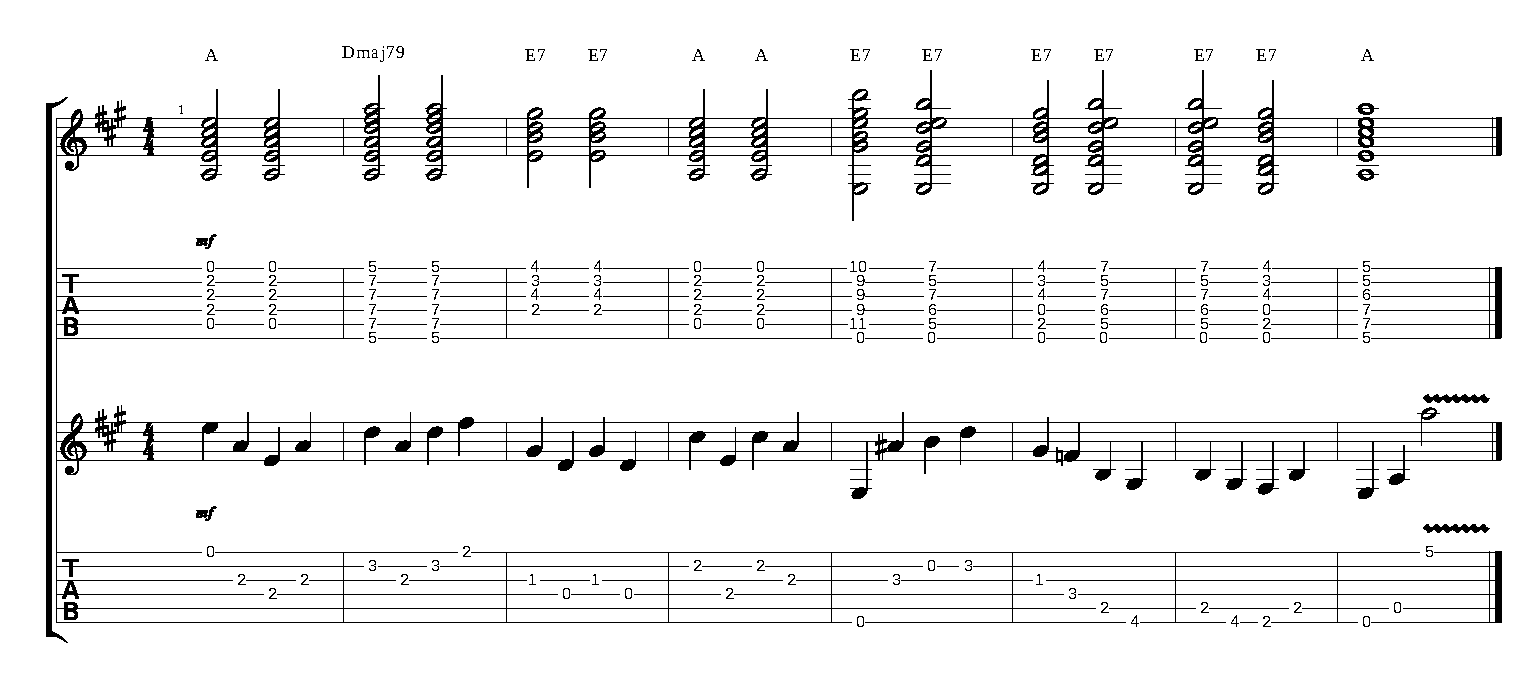
\includegraphics[page=1,scale=0.70]{notes/dallamszerkesztes.pdf}
 \captionof{figure}{Vertikális értelmezéssel színezett dallammenet}
 \label{fig:notevertical}
\end{figure}

\begin{figure}[!htbp]
 \advance\leftskip-6mm
 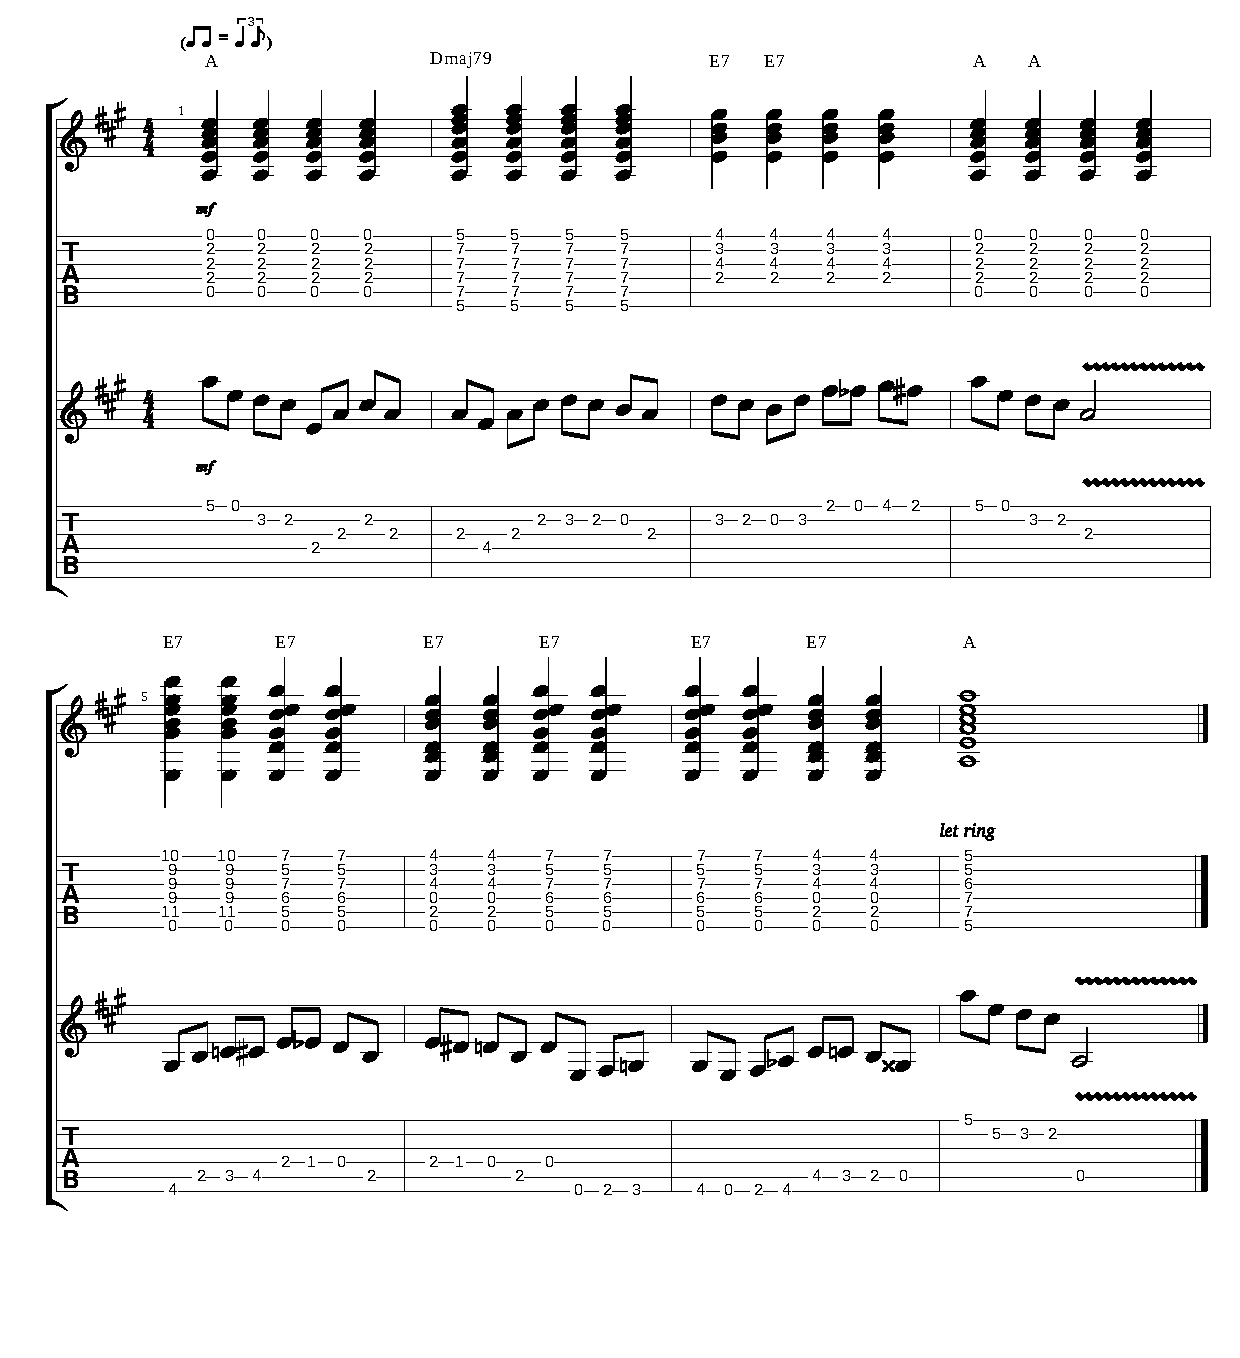
\includegraphics[page=1,scale=0.85]{notes/dallamszerkesztes_II.pdf}
 \captionof{figure}{Enharmonikus kiegészítéssel színezett dallammenet}
 \label{fig:noteenharmonic}
\end{figure}

%
%\stepcounter{section}
%\addcontentsline{toc}{section}{\arabic{section}.~~Ábrajegyzék}
%\label{app:abrajegyzek}
%\listoffigures
%
%\stepcounter{section}
%\addcontentsline{toc}{section}{\arabic{section}.~~Szószedet}
%%\newacronym{Palo}{name={Palo},description={flamenco stílus}}
%\newacronym{Aire}{name={Aire},description={a flamenco által keltett hangulat, a stílus atmoszférája}}
%\newacronym{Pulgar}{name={Pulgar},description={hüvelykujj}}
%\newacronym{Rasgueado}{name={Rasgueado},description={pörgetés technikák összefoglaló neve}}
%\newacronym{Apagado}{name={Apagado},description={némítás bal mutatóujjal, vagy jobb tenyéréllel}}
%\newacronym{Golpe}{name={Golpe},description={kopogás a gitár testén}}
%\newacronym{Golpeador}{name={Golpeador},description={koptatólap a hanglyuk és a híd között}}
%\newacronym{Baile}{name={Baile},description={tánc}}
%\newacronym{Kante}{name={Kante},description={ének}}
%\newacronym{Toka}{name={Toka},description={flamenco gitárjáték}}
%\newacronym{Tokaor}{name={Tokaor},description={flamenco gitáros}}
%\newacronym{Guitarrero}{name={Guitarrero},description={gitárkészítő}}
%\newacronym{Kantaor}{name={Kantaor},description={énekes}}
%\newacronym{Palmaor}{name={Palmaor},description={tapsoló}}
%\newacronym{Bailaor}{name={Bailaor},description={táncos}}
%\newacronym{Apoyando}{name={Apoyando},description={a hüvelykujj pengetés után a következő húrt érinti}}
%\newacronym{Ayudao}{name={Ayudao},description={váltott pengetés hüvelyk- és mutatóujjal}}
%\newacronym{Abanico}{name={Abanico},description={,,legyező'' rasgueado technika}}
%\newacronym{Tremolo}{name={Tremolo},description={PIAMI pengetés sorozat}}
%\newacronym{Anular}{name={Anular},description={gyűrűsujj}}
%\newacronym{Medio}{name={Medio},description={középső ujj}}
%\newacronym{Indíc}{name={Indíc},description={mutatóujj}}
%\newacronym{Alzapúa}{name={Alzapúa},description={több húr kétirányú pengetése hüvelykujjal}}
%

%\printglossaries
%
\section{Melléklet}
\label{sec:melleklet}
\subsection{Skálafokok akkordjai}
\label{sec:skalaakkordok}
\begin{tabular}{llp{18mm}p{17mm}p{18mm}p{17mm}p{18mm}p{17mm}p{18mm}}
\multicolumn{2}{l}{Hangköz} & I & II & III & IV & V & VI & VII \\ \hline \\[-2.2ex]
p  &     & C & D & E & F & G & A & H \\
k2 & k9  &   &   & F'&   &   &   & C'\\
n2 & n9  & D'& E'&   & G'& A'& H'&   \\
k3 & k10 &   & F & G &   &   & C & D \\
n3 & n10 & E &   &   & A & H &   &   \\
t4 & t11 & F'& G'& A'&   & C'& D'& E'\\
b4 & b11 &   &   &   & H'&   &   & F \\
t5 & t12 & G & A & H & C & D & E &   \\
k6 & k13 &   &   & C'&   &   & F'& G'\\
n6 & n13 & A'& H'&   & D'& E'&   &   \\
k7 &     &   & C & D &   & F & G & A \\
n7 &     & H &   &   & E &   &   &   \\ \hline \\[-2.2ex]
\multicolumn{2}{l}{Hármas} &
$C$ & $D_m$ & $E_m$ & $F$ & $G$ & $A_m$ & $H^\dim$ \\[0.4ex]
\multicolumn{2}{l}{Négyes} &
$C^{maj7}$ & $D_m^7$ & $E_m^7$ & $F^{maj7}$ & $G^7$ & $A_m^7$ & $H^\sdim$ \\[0.4ex]
\multicolumn{2}{l}{Ötös} &
$C^{maj9}$ & $D_m^9$ & $E_m^{9b}$ & $F^{maj9}$ & $G^9$ & $A_m^9$ & $H^{\sdim9b}$ \\[0.4ex]
\multicolumn{2}{l}{Hatos} &
$C^{maj11b}$ & $D_m^{11b}$ & $E_m^{9b11b}$ & $F^{maj11}$ & $G^{11b}$ & $A_m^{11b}$ &  $H^{\sdim9b11b}$ \\[0.4ex]
\multicolumn{2}{l}{Hetes} &
$C^{maj11b13}$ & $D_m^{11b13}$ & $E_m^{9b11b13b}$ & $F^{maj13}$ & $G^{11b13}$ & $A_m^{11b13b}$ & $H^{\sdim9b11b13b}$ \\
\end{tabular}
\captionof{figure}{A dúr skála fokaira épülő hangzatok} 
\label{fig:durskalahangzatok}~\\\\
\begin{tabular}{llp{18mm}p{17mm}p{18mm}p{17mm}p{18mm}p{17mm}p{18mm}}
\multicolumn{2}{l}{Hangköz} & I & II & III & IV & V & VI & VII \\ \hline \\[-2.2ex]
p  &     & A     & H     & C     & D     & E     & F     & \gisz \\
k2 & k9  &       & C'    &       &       & F'    &       & A'    \\
n2 & n9  & H'    &       & D'    & E'    &       &       &       \\
k3 & k10 & C     & D     &       & F     &       & \gisz'& H     \\
n3 & n10 &       &       & E     &       & \gisz & A     & C'    \\
t4 & t11 & D'    & E'    & F'    &       & A'    &       &       \\
b4 & b11 &       & F     &       & \gisz'&       & H'    & D     \\
t5 & t12 & E     &       &       & A     & H     & C     &       \\
k6 & k13 & F'    &       & \gisz &       & C'    &       & E'    \\
n6 & n13 &       & \gisz'& A'    & H'    &       & D'    & F     \\
k7 &     &       & A     &       & C     & D     &       &       \\
n7 &     & \gisz &       & H     &       &       & E     &       \\ \hline \\[-2.2ex]
\multicolumn{2}{l}{Hármas} &
$A_m$ & $H^\dim$ & $C^+$ & $D_m$ & $E$ & $F$ & \gisz$^\dim$ \\[0.4ex]
\multicolumn{2}{l}{Négyes} &
$A_m/^{maj7}$ & $H^{\sdim7}$ & $C^{maj7(5\#)}$ & $D_m^7$ & $E^7$ & $F^{maj7}$ & \gisz$^{\dim}$ \\[0.4ex]
\multicolumn{2}{l}{Ötös} &
$A_m/^{maj9}$ & $H^{\sdim9b}$ & $C^{maj9(5\#)}$ & $D_m^9$ & $E^{9b}$ & $F^{maj9\#}$ & \gisz$^{\dim9b}$ \\[0.4ex]
\multicolumn{2}{l}{Hatos} &
$A_m/^{maj11b}$ & $H^{\sdim9b11b}$ & $C^{maj11b(5\#)}$ & $D_m^{11}$ & $E^{9b11b}$ & $F^{maj11\#}$ & \gisz$^{\dim9b11bb}$ \\[0.4ex]
\multicolumn{2}{l}{Hetes} &
$A_m/^{maj11b13b}$ & $H^{\sdim9b11b13}$ & $C^{maj11b13(5\#)}$ & $D_m^{13}$ & $E^{9b11b13b}$ & $F^{maj13\#}$ & \gisz$^{\dim9b11bb13b}$ \\[0.4ex]
\end{tabular}
\captionof{figure}{A (harmonikus) moll skála fokaira épülő hangzatok} 
\label{fig:mollskalahangzatok}~\\\\
\begin{tabular}{llp{18mm}p{17mm}p{18mm}p{17mm}p{18mm}p{17mm}p{18mm}}
\multicolumn{2}{l}{Hangköz} & I & II & III & IV & V & VI & VII \\ \hline
p  &     & A     & H     & C     & D     & E     & \fisz & \gisz \\
k2 & k9  &       & C'    &       &       &       &       & A'    \\
n2 & n9  & H'    &       & D'    & E'    & \fisz'& \gisz'&       \\
k3 & k10 & C     & D     &       &       &       & A     & H     \\
n3 & n10 &       &       & E     & \fisz & \gisz &       & C'    \\
t4 & t11 & D'    & E'    &       &       & A'    & H'    &       \\
b4 & b11 &       &       & \fisz'& \gisz'&       & C     & D     \\
t5 & t12 & E     & \fisz &       & A     & H     &       &       \\
k6 & k13 &       &       & \gisz &       & C'    & D'    & E'    \\
n6 & n13 & \fisz'& \gisz'& A'    & H'    &       &       &       \\
k7 &     &       & A     &       & C     & D     & E     & \fisz \\
n7 &     & \gisz &       & H     &       &       &       &       \\ \hline
\multicolumn{2}{l}{Hármas} &
$A_m$ & $H_m$ & $C^+$ & $D$ & $E$ & \fisz$^\dim$ & \gisz$^\dim$ \\[0.4ex]
\multicolumn{2}{l}{Négyes} &
$A_m/^{maj7}$ & $H_m^7$ & $C^{maj7(5\#)}$ & $D^7$ & $E^7$ & \fisz$^\sdim$ & \gisz$^\sdim$ \\[0.4ex]
\multicolumn{2}{l}{Ötös} &
$A_m/^{maj9}$ & $H_m^{9b}$ & $C^{maj9(5\#)}$ & $D^9$ & $E^9$ & \fisz$^{\sdim9}$ & \gisz$^{\sdim9b}$ \\[0.4ex]
\multicolumn{2}{l}{Hatos} &
$A_m/^{maj11b}$ & $H_m^{9b11b}$ & $C^{maj11(5\#)}$ & $D^{11}$ & $E^{11b}$ & \fisz$^{\sdim11b}$ & \gisz$^{\sdim9b11bb}$ \\[0.4ex]
\multicolumn{2}{l}{Hetes} &
$A_m/^{maj11b13}$ & $H_m^{9b11b13}$ & $C^{maj13(5\#)}$ & $D^{13}$ & $E^{11b13b}$ & \fisz$^{\sdim11b13b}$ & \gisz$^{\sdim9b11bb13b}$ \\[0.4ex]
\end{tabular}
\captionof{figure}{A melodikus moll skála fokaira épülő hangzatok} 
\label{fig:melodikusmollskalahangzatok}~\\\\
\begin{tabular}{llp{18mm}p{17mm}p{18mm}p{17mm}p{18mm}p{17mm}p{18mm}}
\multicolumn{2}{l}{Hangköz} & I & II & III & IV & V & VI & VII \\ \hline \\[-2.2ex]
p  &     & A     & \aisz & C     & D     & E     & F     & G     \\
k2 & k9  & \aisz'&       &       &       & F'    &       &       \\
n2 & n9  &       & C'    & D'    & E'    &       & G'    & A'    \\
k3 & k10 & C     &       &       & F     & G     &       & \aisz \\
n3 & n10 &       & D     & E     &       &       & A     &       \\
t4 & t11 & D'    &       & F'    & G'    & A'    & \aisz'& C'    \\
b4 & b11 &       & E'    &       &       & \aisz &       &       \\
t5 & t12 & E     & F     & G     & A     &       & C     & D     \\
k6 & k13 & F'    &       &       & \aisz'& C'    &       &       \\
n6 & n13 &       & G'    & A'    &       &       & D'    & E'    \\
k7 &     & G     &       & \aisz & C     & D     &       & F     \\
n7 &     &       & A     &       &       &       & E     &       \\ \hline \\[-2.2ex]
\multicolumn{2}{l}{Hármas} &
$A_m$ & \aisz & $C$ & $D_m$ & $E^\dim$ & $F$ & $G_m$ \\[0.4ex]
\multicolumn{2}{l}{Négyes} &
$A_m^7$ & \aisz$^{maj7}$ & $C^7$ & $D_m^7$ & $E^\sdim$ & $F^{maj7}$ & $G_m^7$ \\[0.4ex]
\multicolumn{2}{l}{Ötös} &
$A_m^{9b}$ & \aisz$^{maj9}$ & $C^9$ & $D_m^9$ & $E^{\sdim9b}$ & $F^{maj9}$ & $G_m^9$ \\[0.4ex]
\multicolumn{2}{l}{Hatos} &
$A_m^{9b11b}$ & \aisz$^{maj11}$ & $C^{11b}$ & $D_m^{11b}$ &  $E^{\sdim9b11b}$ & $F^{maj11b}$ & $G_m^{11b}$ \\[0.4ex]
\multicolumn{2}{l}{Hetes} &
$A_m^{9b11b13b}$ & \aisz$^{maj13}$ & $C^{11b13}$ & $D_m^{11b13b}$ & $E^{\sdim9b11b13b}$ & $F^{maj11b13}$ & $G_m^{11b13}$ \\
\end{tabular}
\captionof{figure}{Az A-fríg skála fokaira épülő hangzatok} 
\label{fig:frigskalahangzatok}

%\phantomsection\addcontentsline{toc}{subsection}{A~~Skálák}
\label{app:skalak}
\includepdf[pages=-,pagecommand=\thispagestyle{plain}]{./app_scales.pdf}

\phantomsection\addcontentsline{toc}{subsection}{B~~Akkordok}
\label{app:akkordok}
\includepdf[pages=-,pagecommand=\thispagestyle{plain}]{./app_scales.pdf}

\phantomsection\addcontentsline{toc}{subsection}{C~~Kották}
\label{app:kottak}
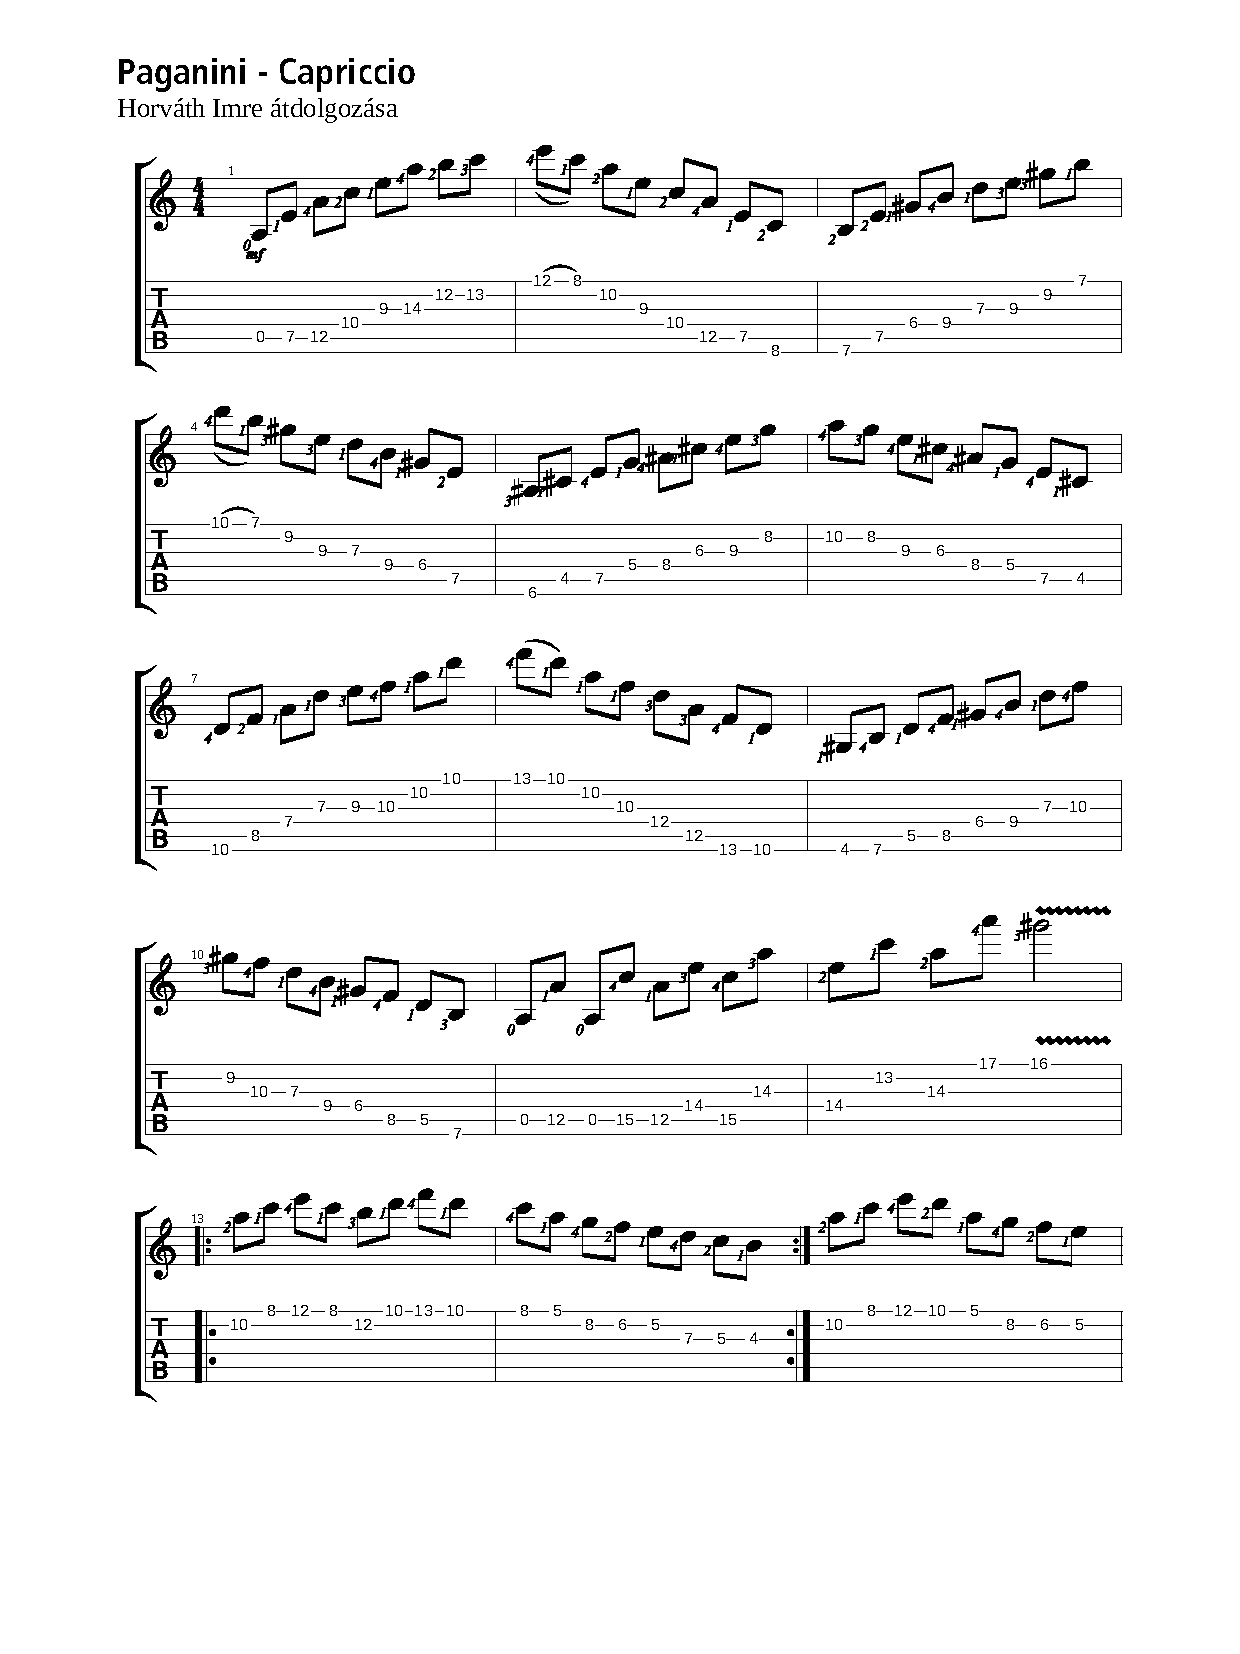
\includepdf[pages=-,pagecommand=\thispagestyle{plain}]{notes/capriccio.pdf}
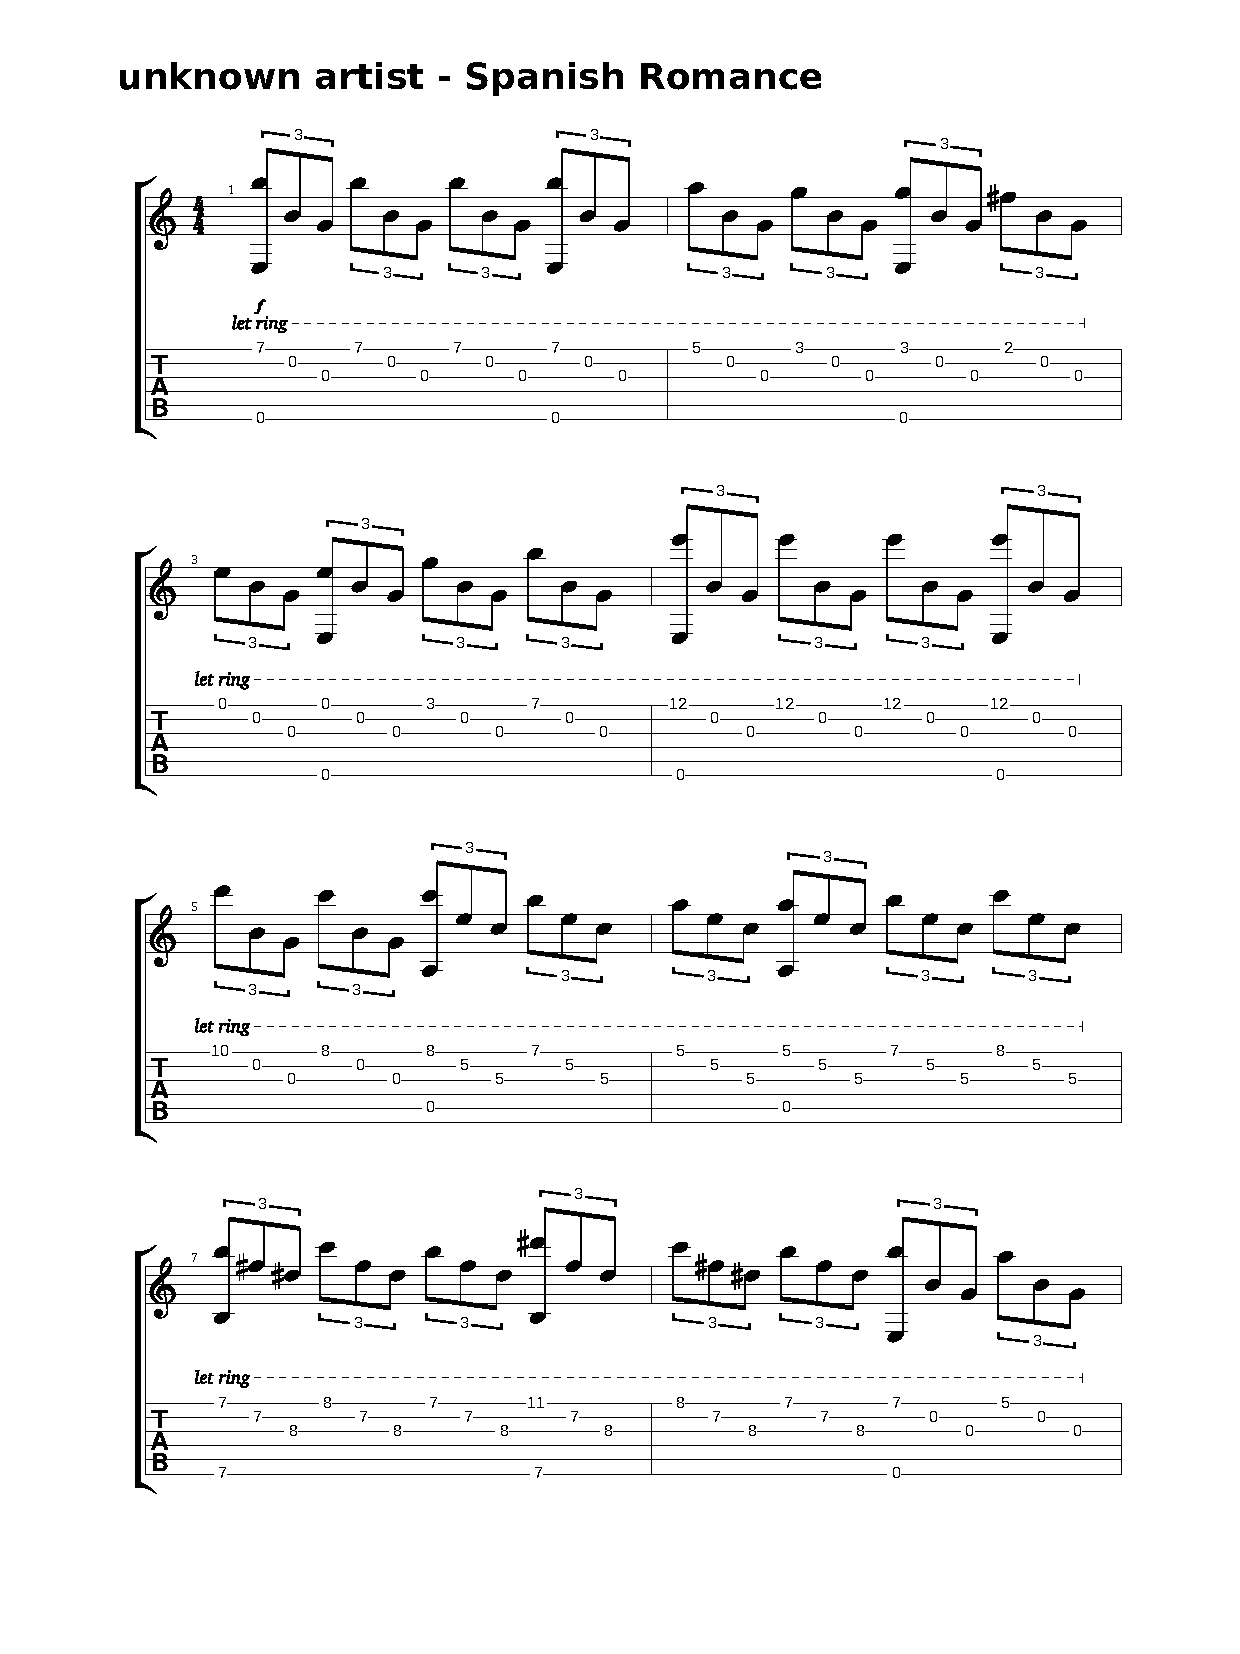
\includepdf[pages=-,pagecommand=\thispagestyle{plain}]{notes/spanishromance.pdf}
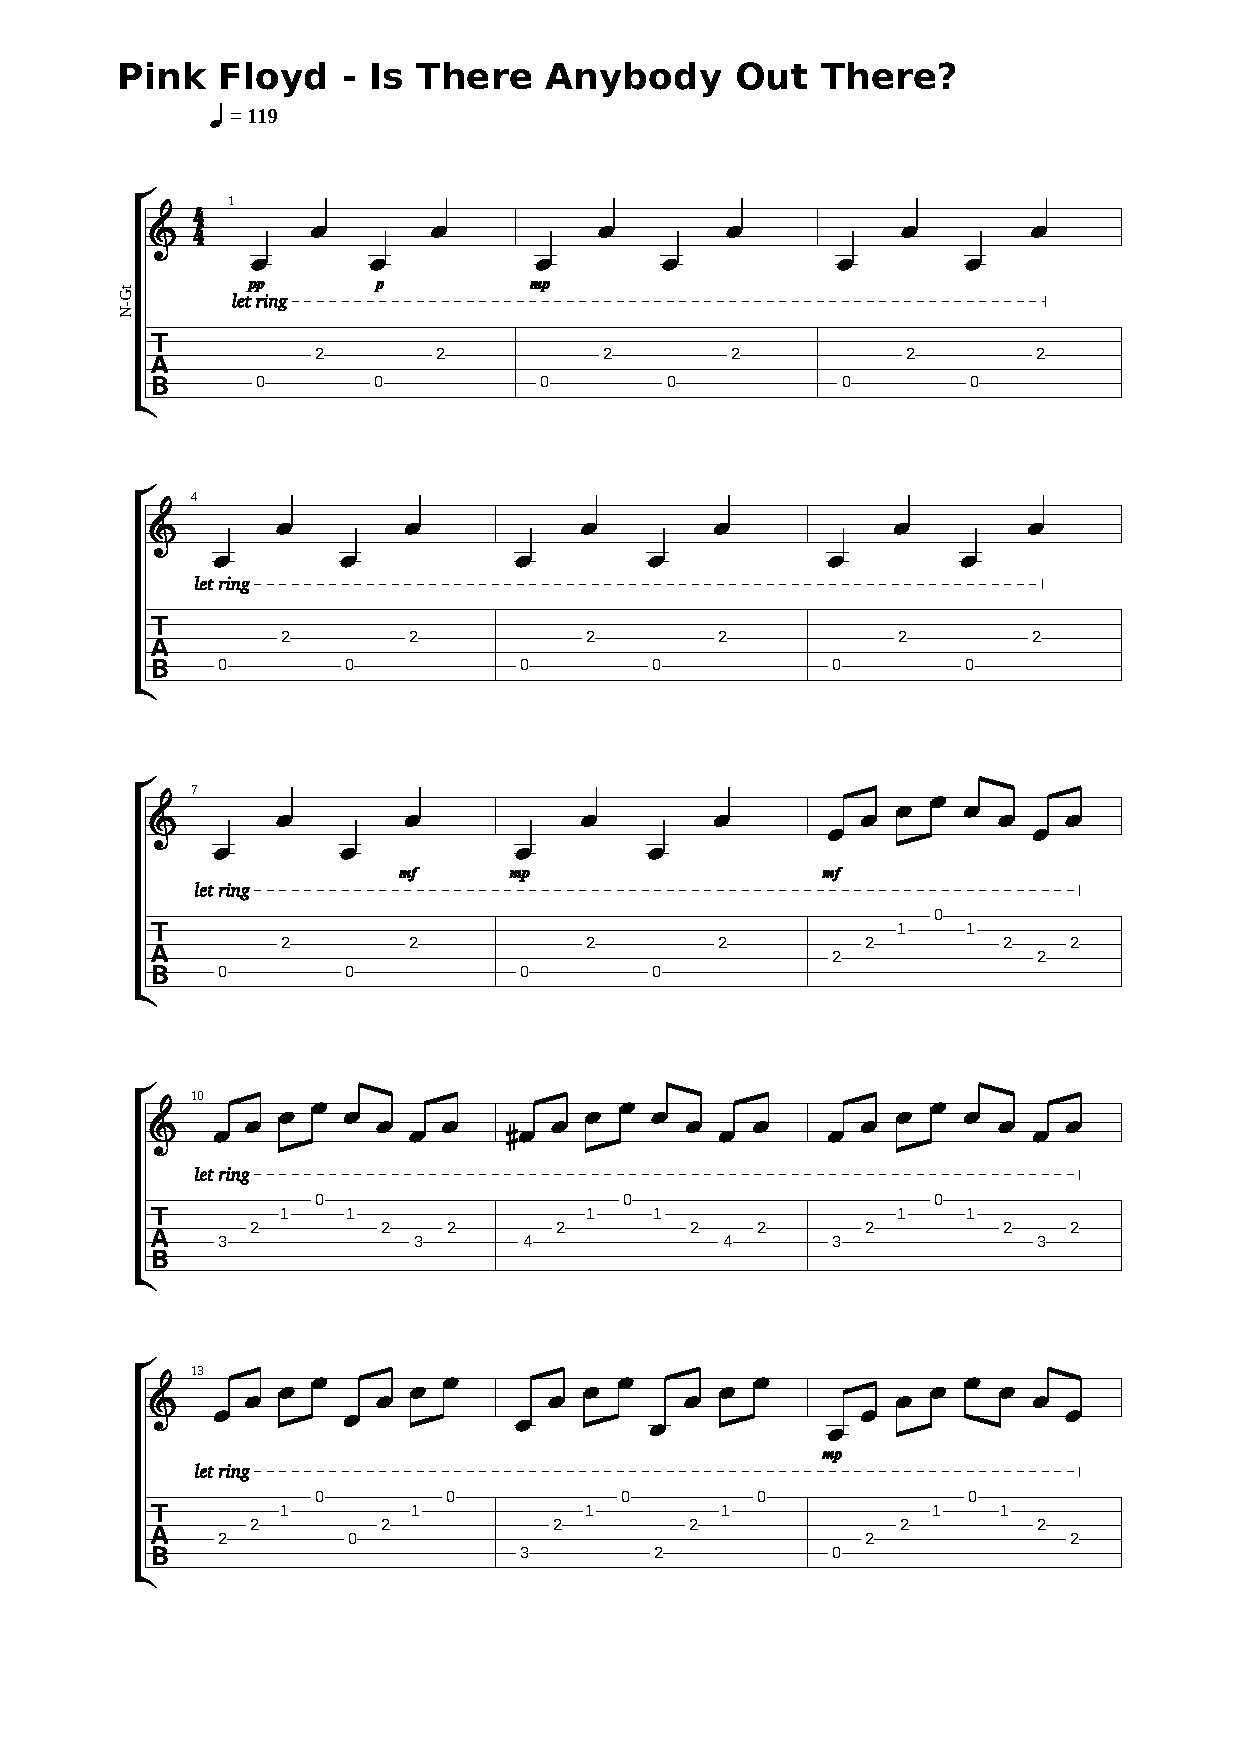
\includepdf[pages=-,pagecommand=\thispagestyle{plain}]{notes/isthereanybodyoutthere.pdf}



\end{document}
